\section{Measurement Methods}

\subsection{General Structure}
\begin{figure}
	\centering
	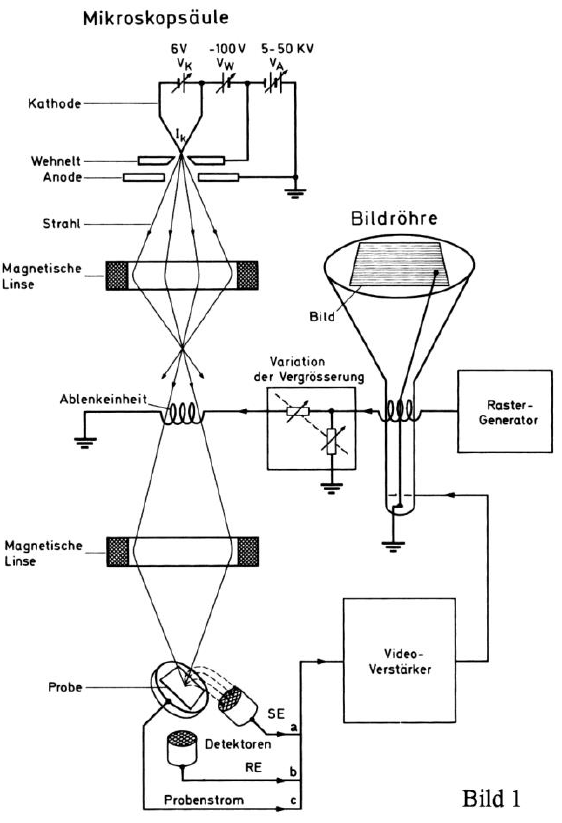
\includegraphics[width=0.95\linewidth]{../assets/aufbau.png}
	\caption{Setup of a scanning electron microscope. \imcite{rem_script}}
	\label{fig:general_structure}
\end{figure}
A schematic	representation of a scanning electron microscope is shown in
\cref{fig:general_structure}.
A cathode emits electrons that are accelerated afterwards by an anode
and focused into a nanometer-wide beam by multiple magnetic lenses.

The goal of a \ac{sem} is to probe the sample at different spots.
To achieve this, one can use the magnetic field of a coil that deflects
the electron beam.
As a result, the electron beam scans across the surface in a raster
pattern. Various detectors are positioned near the sample to measure
different interaction products resulting from the electrons colliding
with the sample atoms. This allows for the generation of an intensity
signal that depends on the position of the electron beam.

For older devices, the electron beam position is synchronized
with a CRT.
In newer devices, the signal is digitized and can be outputted in
various formats.

\subsection{Electron Beam Generation}
Electrons can be produced via thermionic emission, such as with a tungsten hairpin cathode that is used in this experiment.
The cathode is heated to a temperature range of
\qtyrange{2600}{3000}{\kelvin} to overcome the work function of
\qty{2.5}{\electronvolt} through thermal excitation.
The cathode is surrounded by a Wehnelt-cylinder, on which a voltage is
applied.
The cylinder is used as a first focusing mechanism.
This is schematically visualized in \cref{fig:wolfram}.
\begin{figure}
	\centering
	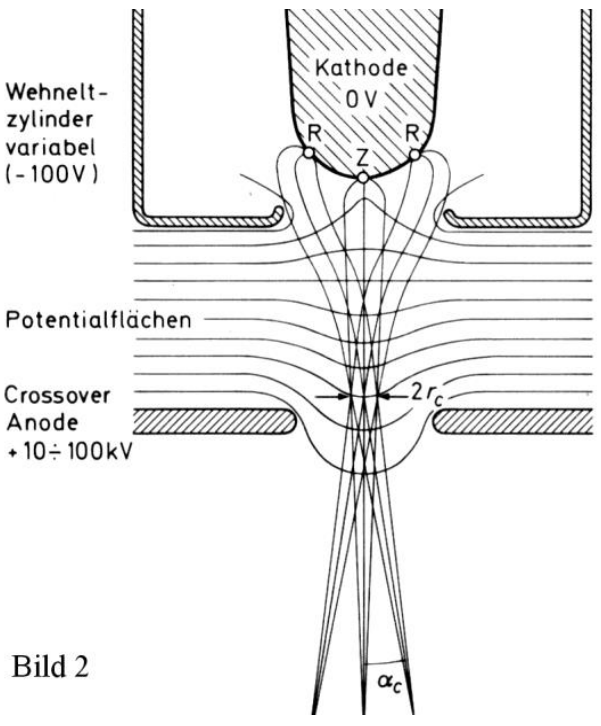
\includegraphics[width=0.95\linewidth]{../assets/wolfram.png}
	\caption{Geometric arrangement of the cathode and the Wehnelt-cylinder.
		\imcite{rem_script}}
	\label{fig:wolfram}
\end{figure}
There also exist \ce{LaB6} cathodes, which consist of a small rod-shaped
lanthanum hexaboride single crystal.
This crystal is indirectly heated to temperature ranging
from \qtyrange{1700}{2100}{\kelvin}.
Due to the lower work function of \qty{2.7}{\electronvolt} the cathode
can work at a lower temperature.

Apart from thermionic emission, there also exist field emission, where
the quantum mechanical tunneling effect is utilized to generate electrons.
This provides a more precise beam but is also more complex to operate.

\subsection{Electron Lenses}
After being emitted by the cathode, the electron beam cross-section
needs to be reduced further.
To achieve this, electron lenses are used.
The most common architecture is a magnetic coil that generates a
rotationally symmetric field.
The field amplitude is gaussian-shaped along the symmetry axis.
When electrons arrive at the coil, they are forced to move in a helix
trajectory and merged into the focal point.

As with optical lenses, electron lenses show a variety of
aberrations, which need to be considered.
\begin{itemize}
	\item \textit{Spherical aberration} occurs because off-axis electrons
	      are deflected more strongly than on-axis electrons, resulting in a
	      shorter focal point. Spherical aberration increases at large
	      aperture angles.
	\item \textit{Axial astigmatism} is an imaging error related to the
	      magnetic inhomogenities, that leads to a deviation from rotational
	      symmetry.
	      This deviation causes different focal points for different beam
	      planes.
	\item \textit{Chromatic errors} are another type of aberration
	      which originates from the velocity distribution of the electrons.
	      Different velocities result in different wavelengths and different
	      focal points.
	\item \textit{Diffraction errors} occur because of the small aperture
	      angle and the resulting single slit interference of electron waves.
	      This leads to a blurred lens focus.
	      As diffraction errors increase with small aperture angles and
	      spherical aberrations increase with large angles, one can find an
	      optimal angle that minimizes the total error.
\end{itemize}
